\documentclass[twocolumn]{bmcart}

\usepackage{fontspec}
\usepackage{csquotes}
\usepackage{polyglossia}
\usepackage{hyperref}
\usepackage{pgf,tikz}
\usepackage{mathrsfs}
\usetikzlibrary{arrows}
\usepackage{pstricks-add}
\usepackage{float}
\usepackage{afterpage}
\usepackage{amsmath}
\usepackage{amssymb}
\makeatletter
\afterpage{\global\setlength\@fpsep{8\p@ \@plus 2fil}}
\makeatother
\renewcommand{\floatpagefraction}{0.1}
\newenvironment{equations}{\equation\aligned}{\endaligned\endequation}


\setmainlanguage{german}
\makeatletter
\@fpsep\textheight
\makeatother

\usepackage{graphicx} % for pdf, bitmapped graphics files
%\usepackage{caption}
%\usepackage{subcaption}
\usepackage{listings}
\usepackage{framed}

%\usepackage{xcolor}

\colorlet{shadecolor}{gray!20}

\lstnewenvironment{mat}
{\lstset{language=mathematica,mathescape,columns=flexible}}
{}

\lstset{language=Mathematica}
\lstset{basicstyle={\sffamily\footnotesize},
	numbers=left,
	numberstyle=\tiny\color{gray},
	numbersep=5pt,
	breaklines=true,
	captionpos={t},
	frame={lines},
	rulecolor=\color{black},
	framerule=0.5pt,
	columns=flexible,
	tabsize=2
}



%%% Begin ...
\begin{document}
	
	%%% Start of article front matter
	\begin{frontmatter}
		
		\begin{fmbox}
			\dochead{Topoi Forschung}

%%%%%%%%%%%%%%%%%%%%%%%%%%%%%%%%%%%%%%%%%%%%%%
%%                                          %%
%% Enter the authors here                   %%
%%                                          %%
%% Specify information, if available,       %%
%% in the form:                             %%
%%   <key>={<id1>,<id2>}                    %%
%%   <key>=                                 %%
%% Comment or delete the keys which are     %%
%% not used. Repeat \author command as much %%
%% as required.                             %%
%%                                          %%
%%%%%%%%%%%%%%%%%%%%%%%%%%%%%%%%%%%%%%%%%%%%%%

\author[
addressref={aff1,aff2,aff3},                   % id's of addresses, e.g. {aff1,aff2}
corref={aff1},                       % id of corresponding address, if any
%noteref={n1},                        % id's of article notes, if any
email={gerd.grasshoff@hu-berlin.de}   % email address
]{\inits{}\fnm{Gerd} \snm{Graßhoff}}
\author[
addressref={aff2},
email={gordon.fischer@topoi.org}
]{\inits{}\fnm{Gordon} \snm{Fischer}}

%%%%%%%%%%%%%%%%%%%%%%%%%%%%%%%%%%%%%%%%%%%%%%
%%                                          %%
%% Enter the authors' addresses here        %%
%%                                          %%
%% Repeat \address commands as much as      %%
%% required.                                %%
%%                                          %%
%%%%%%%%%%%%%%%%%%%%%%%%%%%%%%%%%%%%%%%%%%%%%%

\address[id=aff1]{%                           % unique id
	\orgname{Institut für Philosophie, Humboldt Universität zu Berlin}, % university, etc
	\street{Unter den Linden 6},                     %
	\postcode{10099}                                % post or zip code
	\city{Berlin},                              % city
	\cny{Deutschland}                                    % country
}
\address[id=aff2]{%
	\orgname{Excellence Cluster Topoi, Hannoversche Str. 6, Humboldt Universität zu Berlin},
	\street{Hannoversche Str. 6},
	\postcode{10099}
	\city{Berlin},
	\cny{Deutschland}
}
\address[id=aff3]{%
	\orgname{Max-Planck-Institut für Wissenschaftsgeschichte},
	\street{Boltzmannstr. 22},
	\postcode{14195}
	\city{Berlin},
	\cny{Deutschland}
}

%%%%%%%%%%%%%%%%%%%%%%%%%%%%%%%%%%%%%%%%%%%%%%
%%                                          %%
%% Enter short notes here                   %%
%%                                          %%
%% Short notes will be after addresses      %%
%% on first page.                           %%
%%                                          %%
%%%%%%%%%%%%%%%%%%%%%%%%%%%%%%%%%%%%%%%%%%%%%%

\begin{artnotes}
	%\note{Sample of title note}     % note to the article
	\note[id=n1]{Equal contributor} % note, connected to author
\end{artnotes}

\end{fmbox}% comment this for two column layout
%%%%%%%%%%%%%%%%%%%%%%%%%%%%%%%%%%%%%%%%%%%%%%
%%                                          %%
%% The Abstract begins here                 %%
%%                                          %%
%% Please refer to the Instructions for     %%
%% authors on http://www.biomedcentral.com  %%
%% and include the section headings         %%
%% accordingly for your article type.       %%
%%                                          %%
%%%%%%%%%%%%%%%%%%%%%%%%%%%%%%%%%%%%%%%%%%%%%%

\begin{abstractbox}
	
	\begin{abstract} % abstract

	\end{abstract}
	
	%%%%%%%%%%%%%%%%%%%%%%%%%%%%%%%%%%%%%%%%%%%%%%
	%%                                          %%
	%% The keywords begin here                  %%
	%%                                          %%
	%% Put each keyword in separate \kwd{}.     %%
	%%                                          %%
	%%%%%%%%%%%%%%%%%%%%%%%%%%%%%%%%%%%%%%%%%%%%%%
	
	\begin{keyword}
		\kwd{Aphrodisias}
		\kwd{Bauzeichnung}
		\kwd{Entasis}
	\end{keyword}
	
	% MSC classifications codes, if any
	%\begin{keyword}[class=AMS]
	%\kwd[Primary ]{}
	%\kwd{}
	%\kwd[; secondary ]{}
	%\end{keyword}
	
\end{abstractbox}
%
%\end{fmbox}% uncomment this for twcolumn layout
Eine Bauzeichnung antiker Säulen aus dem  hinteren Bühnenbereich  des Theaters von Aphrodisias  wird mit modernen fotogrammetrischen Methoden aufgenommen und ihre Geometrie vermessen. Die geometrischen Eigenschaften der Zeichnung beschreibt eine neuartige Konstruktion ionischer Säulen, die sich von der Bauzeichnungen aus Didyma konzeptionell unterscheidet. Zudem konnte eine am Ort aufgefundene Säule identifiziert werden, deren charakteristische Form mit der Bauzeichnung  übereinstimmt. Damit ist erstmalig der Zusammenhang zwischen einer antiken Säule und der zu ihrer Herstellung genutzten Bauzeichnung hergestellt worden. Die Säulenform erweist sich als überraschend komplex: Die Säule zeigt nicht nur eine neue Variante der Entasis, sie weicht von der Rotationssymmetrie ab. Damit ist erstmalig an einer ionischen Säule eine der Kurvatur vergleichbare Verfeinerung ästhetischer Bauform nachgewiesen.

\end{frontmatter}



\title{Antike Säulen und ihre Konstruktionszeichnung im antiken Aphrodisias}


\date{\today}% It is always \today, today, % but any date may be


\tableofcontents



\maketitle


%%%%%%%%%%%%%%%%%%%%%%%%%%%%%%%%%%%%%%%%%%%%%%%%%%%%%%%%%%%%%%%%%%%%%%%%%%%%%%%%

\thispagestyle{empty}

%%%%%%%%%%%%%%%%%%%%%%%%%%%%%%%%%%%%%%%%%%%%%%%%%%%%%%%%%%%%%%%%%%%%%%%%%%%%%%%%
\section{Einleitung}



Nachdem Lothar Haselberger Bauzeichnungen von Säulen im antiken  Didyma identifizierte \cite{haselbergerlothar1980},  wuchs das Interesse an Bauzeichnungen und geometrischem Wissen antiker Baumeister \cite{haselbergerlothar1999}, \cite{rennjurgen-1}. Trotz aller Bemühungen konnte man bislang keine Konstruktionszeichnungen einer tatsächlich hergestellten  Säule zuordnen. Eine Bauzeichnung von Säulen wurde zwar in der \textit{scaenae frons} des Theaters von Aphrodisias gefunden und publiziert, doch als einfache Konstruktionsvorschrift einer schlichten Säulenform gedeutet.  

\textit{1965 fasste Kenan Erim  den Plan, den Theaterbereich von Aphrodisias auszugraben \cite[p. 7]{smith1991}, mussten  Teile der modernen Stadt Geyre umgesiedelt werden. Dabei wurden 2-8 m Schutt abgetragen. In den siebziger und achtziger Jahren gruben die Archäologen den Theaterbereich aus, in dem sich die hier diskutierten Bauzeichnungen im hinteren Bühnenbereich befinden \cite[p. 7]{smith1991}. Joyce M. Reynolds schlägt für die Datierung des Bühnenbereiches als erste Phase zum Bau des Theaters nach den datierten Inschriften das Jahr 28 B.C. vor \cite[p. 15]{reynolds1991}.
Möglich ist aber auch eine bis zu zwei Jahrhunderte spätere Zeichnung. Die in Position 43 aufgefundene Säule ist nicht unbedingt in der ursprünglichen Orientierung aufgestellt gewesen (NEUE ABBILDUNG!?). Aus dem vorläufigen Grabungsbericht ist das nicht zu entnehmen.}

\begin{figure*}
\centering
\includegraphics[width=1.2\linewidth]{figures/screenshot005}
\caption{Theater Komplex. Die Bauzeichnungen befinden sich an der Wand zu den hinteren Bühnenräumen nahe Punkt 7. Die passende Säule an der Position 43.}
\label{fig:screenshot005}
\end{figure*}

Im Herbst 2015 haben wir die Bauzeichnungen  von Säulen in Aphrodisias während einer Kampagne zur  Erfassung von Sonnenuhren  fotografisch aufgenommen  und ein Netz von vermessenen Referenzpunkten zu Registrierung der Fotos erstellt.

\subsection{Bauzeichnungen}

Unter dem Eindruck der von Haselberger gefundenen Ritzzeichnungen  am  Adyton von Didyma differenziert Heisel verschiedenste Funktionen von Ritzzeichnungen für einen Bau \cite{heisel1993}. Hellenistische Detailrisse sind  Orthogonalprojektionen. Aufrisse und Horizontalschnitte beschreiben die geometrischen Eigenschaften von Bauelementen. Detailrisse zeigen Grundformen der Objekte, wobei unklar bleibt, ob damit Ansichten der Objektformen gemeint sind oder Schnitte durch architektonische Körper. Die von Haselberger gefundene  Risszeichnung einer Säule \href{http://dx.doi.org/10.17171/2-1-8}{\textit{doi:10.17171/2-1-8}} stellt diese in Originalmaßen in der horizontalen Dimension und um den Faktor 16 verkleinerter Vertikale dar. Angedacht war dies für die geometrische Konstruktion der Entasis, die in der verkleinerten Säulenzeichnung als Kreisbogen abgetragen wurde, um in der proportional expandierten Gestalt des Säulenschaft zu einen eleganten elliptischen Querschnittsform zu expandieren. Untersuchungen der Säulen des Pantheon in Rom haben gezeigt, dass dessen Säulen des Portikus eine eben solche elliptische Entasis haben \cite{grasshoffdecoding2013}.

\subsection{Zeichnung von Aphrodisias}

\begin{figure*}
	\centering
	\includegraphics[width=1\linewidth]{figures/screenshot002}
	\caption{\cite{jonesmarkwilson2000}, p. 129, Wandzeichnungen an der hinteren Bühnenraum des Theaters von Aphrodisias.}
	\label{fig:screenshot002}
\end{figure*}

Auf den ersten Blick handelt es sich um eine sehr schlichte, im Maßstab eins zu eins angefertigte Zeichnung einer Säule, deren Geometrie zudem alles andere als genau angelegt scheint. Das in die Zeichnung später eingeritzte Graffiti vermittelt den Eindruck einer nicht sehr komplexen Vorlage für eine Bauzeichnung. So ist es kein Wunder, dass Mark Wilson Jones dieser Zeichnung keinen besonders hohen Stellenwert gibt.

\begin{quotation}{\footnotesize
On the other hand, it is apparent even to the naked eye that shafts belonging to the propylon of the sanctuary at Baalbek and the Hadrianeum in Rome do not curve at all. Measurements of the latter reveal a cranked profile uncannily like Alberti’s; the lower part rises vertically and the upper part tapers in a straight line. It is true that there is a transitional curve between these linear sections, as well as hints of curvature at the very top and bottom, but these are minor adjustments aimed at creating a fluent effect. This method too has now been confirmed by ancient working drawings. The most complete example belongs to the \textit{scaenae frons} of the theatre at Aphrodisias, while a few scratched lines at Pergamon suggest a similar approach. The Aphrodisias drawing defines the outline of a small shaft by just pairs of lines at an oblique angle to one another. The result may be simplistic, but it is hard to imagine anything easier to execute.\cite[p. 128]{jonesmarkwilson2000}}
\end{quotation}

Die Zeichnung stellt demnach einen Säulentyp dar, der mittels zueinander geneigter und geradliniger Strecken, leicht auszuführen wäre. Eine solche Säule ist in Aphrodisias nicht gefunden worden. Auch eine Geländesichtung im September 2015 hat keine so schlicht gebaute Säule auffinden lassen. Der Aufwand für die Erstellung einer Bauzeichnung ist viel zu hoch für eine so einfache Konstruktion. Zwar ist die Zeichenfläche an einer zwar für den Zuschauer des Theaters verborgenen Stelle angebracht, doch ist die nutzbare Wandfläche kostbar. Zudem ist an der gesamten hinteren Wandfläche keine andere Konstruktionszeichnung dieser Art aufgebracht. Die Zeichnungen selbst sind detailliert ausgeführt und zeigen mehrere Pläne übereinandergelegt. Alle Säulen in der Nähe des Theaters zeigen eine Entasis, die mit der direkten geradlinigen Formgestaltung der Zeichnung unverträglich ist. Deshalb ist in Erwägung zu ziehen, dass die geometrische Gestalt der Abbildung keine direkte Formwiedergabe einer Säule ist. In Betracht zu ziehen ist ein vermittelndes Übertragungsverfahren der Zeichnung auf eine Säule. Das Diagramm stellt in einem solchen Verfahren gewisse Grundaspekte der Säule dar, die durch geeignete Wahl modularer Einheiten auf verschiedene Größen skaliert und durch weitere Formelemente wie eine Entasis zu ihrer endgültigen Gestalt gebracht werden können. Zur Konstruktion einer trapezförmigen Säule wäre kaum eine derart aufwendige Bauzeichnung an so prominenter Stelle erforderlich gewesen.


\section{Datenpublikation Edition Topoi}

 Um die für die weitgehende Analyse benutzten Forschungsdaten nachvollziehbar zu machen, publizieren wir die gesamte Datenaufnahme in Gestalt der Fotos, der Messwerte, und der 3D Modellierung der Säule auf der Forschungsplattform \textit{Edition Topoi}\footnote{\href{http://www.edition-topoi.org/}{http://www.edition-topoi.org}}. Wir hoffen damit Anregungen für eigene Datenauswertungsverfahren, fotogrammetrischen Techniken und die Auswertungsmethoden von 3D Modellen geben zu können. Wir erwarten bei diesem wichtigen Fund auch die baldige Erweiterung der Datenaufnahme anderer Säulen in Aphrodisias, um deren genaue Formeigenschaften zu bestimmen und möglicherweise auch der statistischen Analyse zuzuführen.
 
  Alle Forschungsdaten werden in dem Repositorium dauerhaft archiviert, erhalten eine \textit{DOI}\footnote{\href{https://www.doi.org/}{https://www.doi.org/}} Kennzeichnung und sind als Forschungsdaten in Form des neuen Publikationsmediums \textit{Citable}\footnote{\href{http://www.edition-topoi.org/publishing_with_us/citable}{http://www.edition-topoi.org/publishing\_with\_us/citable}} maschinell lesbar und über eine REST-API  entweder direkt digital über das Internet zu laden oder direkt in entsprechende Tools und Arbeitsplattformen einzulesen. Die wissenschaftliche Nutzung der Daten ist im Tausch gegen eine Zitation bei jeder Publikation anzugeben.

Auf der Publikationsplattform \textit{Edition Topoi} sind die Forschungsdaten für die Rekonstruktion der Bauzeichnungen in Aphrodisias veröffentlicht. Dazu gehören die fotografischen Aufnahmen des Bereichs der Wand mit den Zeichnungen, wie auch die Aufnahmen der Säule vor dem Theaterbereich, die Grundlage für die 3D Modellierung sind. Die 3D Modelle selbst sind ebenfalls mit der \textit{Edition Topoi} publiziert. Die \textit{Edition Topoi} hat eine offene maschinenlesbare Schnittstelle, die es erlaubt, aus Programmumgebungen, wie z.B. \texttt{Mathematica}\footnote{\href{http://www.wolfram.com/}{http://www.wolfram.com/}} die Daten einzulesen und weiter zu verarbeiten. In einem ersten Schritt werden die \textit{Citables} der auszuwertenden Fotos geladen (hier \texttt{Mathematica}):


	\begin{shaded}
		\begin{mat}
        In[1]:	Citable = LoadCitable[$\text{10.17171/2-1-2}$];
        In[2]:  image1 = LoadData[Citable,1]
        In[3]:  image2 = LoadData[Citable,2]
		.........
		\end{mat}
	\end{shaded}

In Abb. \ref{img6} zwei Fotos (eine Gesamtaufnahme der Zeichnung und ein vergrößerter Detailausschnitt), an dem die Berechnungen vorgeführt werden.



\section{Fotogrammetrische Vermessung}

Mithilfe einer einfachen Funktion können korrespondierende Punkte gefunden werden (ebenfalls in \texttt{Mathematica}):
    

	\begin{shaded}
		\begin{mat}
 In[1]:  matches = ImageCorrespondingPoints[image1, image2, MaxFeatures -> 10];
 In[2]:  showMatches[image1, image2, matches]
		\end{mat}
    \end{shaded}
    
    
    %\begin{shaded}
%		\begin{mat}
%  In[1]:  	MapThread[HighlightImage[#1, #2] &, {{image1, image2}, ImageCorrespondingPoints[image1, image2]}]
%	    \end{mat}
 %   \end{shaded}
    
\begin{figure*}
	\includegraphics[width=0.5\linewidth]{figures/image1.jpg}
	\includegraphics[width=1.5\linewidth]{figures/image2.jpg}
	\label{img6}
	\caption{Das obere Bild ist ein Ausschnitt aus der unteren Gesamtaufnahme der Konstruktionszeichnung. Mathematica sucht übereinstimmende Punkte auf beiden Bildern, die in Pixelkoordinaten ausgegeben werden.}
\end{figure*}
	
Zur Datenaufnahme der geometrischen  Eigenschaften von Diagrammen auf einer zu vermessenden Fläche eignen sich fotogrammetrische Methoden für digitale Fotographie \cite{kraus2004}. Die Aufgabe besteht darin, eine Pixelkoordinate eines Punktes in die korrespondierende Realkoordinate zu berechnen. Die erforderlichen Transformation sind mittlerweile für viele Anwendungsfälle digitaler Verfahren entwickelt und in Standardprogrammen implementiert worden. Für unseren Fall können wir die Aufgabenstellung dadurch reduzieren, dass wir die eben auf die Wand abgetragenen Diagramme durch eine zweidimensionale Ebene annähern. Die Aufgabe des Messverfahrens  besteht dann darin, die mit Digitalfotos aufgenommenen Bereiche der Wand durch Transformation auf die zweidimensionale Ebene der von uns ``Realkoordinaten'' genannten Zeichnungsebene umzurechnen. Für die Berechnung dieser Transformation verwenden wir in \texttt{Mathematica} implementierte Verfahren des "image processing". Alternativ dazu könnte man die Genauigkeit der Proklamation der Wandfläche mit einer zweidimensionalen geometrischen Ebene durch eine 3D Modellierung prüfen. Dazu werden die digitalen Aufnahmen mit den Methoden der "Structure-from-motion" und dem Programm Fotoscan von Agisoft modelliert und die vermessenen und Referenzpunkte registriert. 

Ziel des hier beschriebenen fotogrammetrischen Verfahrens ist eine sehr detaillierte und gleichzeitig präzise Auswertung der Konstruktionszeichnung zu erstellen. Zuerst sollen dazu fotografische Aufnahmen verwendet werden, um die Bauaufnahme dokumentieren zu können. Das Messverfahren soll die Markierungen mit einer Genauigkeit besser als 1 mm aufnehmen. Das hier beschriebene Verfahren kombiniert dazu moderne fotogrammetrische Methoden der Auswertung von Digitalfotos mit digital vermessenen Messpunkten auf der Wandfläche.

Die Verwendung von verschiedenen hoch aufgelösten Fotos unterschiedlicher Detailauflösung erlaubt es, sehr detailreiche Makroaufnahmen von einzelnen Aspekten der fotografierten Zeichnung mit Übersichtsfotos zu kombinieren und die Verfahren der Digitalfotografie zu verwenden, um die dargestellten Realkoordinaten eines hochaufgelösten digitalen Fotos zu berechnen. Durch diese Technik gelingt es, detailreiche Aufnahmen einzelner fotografischer Aspekte mittels \texttt{Mathematica} in die entsprechenden Realkoordinaten umzurechnen. Die Python-Bibliothek scikit-image verwendet ähnliche Verfahren.\footnote{\href{http://scikit-image.org/}{Python library scikit.}}


\subsection{Feature detection and correlation}


Im ersten Schritt werden charakteristische Eigenschaften in den Fotos markiert. 
\texttt{Mathematica} verwendet ein "feature detection" Verfahren, um sie maschinellen zu identifizieren. In dem Beispiel aus Abb. \ref{img6} beschränken wir die zu berechnende Zahl der Merkmale auf zehn. 

Korrespondierende Merkmale von Vergleichsfotos legen die aufeinander abzubildenden gleichen Stützpunkte der Fotos fest. Dazu verwendet \texttt{Mathematica} ein robustes Verfahren der fehlertoleranten Zuordnung korrespondierender Merkmale.\footnote{Gut beschrieben in scikit.image} Diese Merkmale  lassen die zugehörigen Transformationen für die Zuordnungen der Fotos berechnen. 

\subsection{Image registration}

Zwei Bilder mit korrespondierenden Markierungen sollen so aufeinander abgebildet werden, dass eine Transformationsfunktion vom  Koordinatensystem des einen Bildes auf das Koordinatensystem des anderen, und am Schluss alle Bildkoordinatensysteme auf das Koordinatensystem der fotografierten Zeichenfläche umgerechnet werden kann. 

Es ergeben sich zwei Punktmengen \texttt{R} für die Referenzpunkte und \texttt{P} für die Pixelkoordinaten mit jeweils \texttt{n} Punktepaaren, die in einer Beziehung zueinander stehen. Für diese kann in  \texttt{Mathematica} eine Transformationsvorschrift gefunden werden:

\begin{equation}
({err, \mbox{TransformationFunction}[
\begin{pmatrix}
a_1 & a_2 & a_3  \\
b_1 & b_2 & b_3  \\
c_1 & c_2 & c_3 
\end{pmatrix}
  ])}
\end{equation} 

mit dem angenommenen mittleren Fehler der Überlagerung \texttt{err} und den Werten \texttt{$a_1$} bis \texttt{$c_3$} für die Umwandlung eines Punktes $R_n(x,y)$ in einen Punkt $P_n(x,y)$.

Diese Verfahren werden auch unter dem Begriff der Image Registration in der Literatur ausführlich behandelt.\footnote{Siehe \href{https://en.wikipedia.org/wiki/Imageregistration}{Image registration (Wikipedia)} und point set registration \href{https://en.wikipedia.org/wiki/Pointsetregistration}{point set registration (Wikipedia)}.}

Die vermessenen Messpunkte auf der Wandfläche werden mit \texttt{Mathematica} ausgewertet und daraus optimierte Referenzkoordinaten  berechnet. Die ermittelten Koordinaten der Referenzpunkte werden so gewählt, dass die Summe über die Fehlerquadrate der vermessenen Distanzen zwischen den Referenzpunkten  minimiert wird:
\begin{equation}
\sum^i [(d^{calculated}_i)^2 - (d^{measured}_i)^2] \rightarrow 0.
\end{equation}
Dieses Koordinatensystem definiert sogenannte Realkoordinaten der Messfläche. Die Messpunkte wurden vor Ort durch kleine Aufkleber auf der Wand markiert. Eine hinreichend große Anzahl  der so markierten Messpunkten erlaubt es, auch sehr fein auflösende Detailfotos mit entsprechenden Transformationsfunktionen auf die Realkoordinaten umzurechnen.

\begin{figure*}
	\centering
	\includegraphics[width=1\linewidth]{figures/Messpunktnetz.pdf}
	\caption{Netz von Messpunkten über die gesamte Konstruktionszeichnung.an der Wand im hinteren Theaterbereich von Aphrodisias.}
	\label{fig:messpunktnetz}
\end{figure*}

Die für die Registrierung verwendeten Bilder können unter \href{http://dx.doi.org/10.17171/2-1-2}{\textit{doi:10.17171/2-1-2}} aufgerufen werden.

Das Netzwerk der vermessenen Messpunkte zeigt die Abb. \ref{fig:messpunktnetz}. Die einzelnen  gemessenen Distanzen zwischen Referenzpunkten sind mit einem Laserdistanzmesser manuell  mit einer Genauigkeit weit unter 1 mm vermessen worden. Durch die Minimierung der Abweichung Quadrate mittels  \texttt{Mathematica} dürften die resultierenden Genauigkeiten der Positionsmessungen noch weiter gesteigert worden sein.

Mit den so erhaltenen Koordinaten der Referenzpunkte lassen sich durch ein oben beschriebenes Verfahren die Transformationsfunktionen berechnen, die von einem Übersichtsfoto und den darauf bestimmten Markierungen der Referenzpunkte die Umrechnungen auf die Realkoordinaten des Referenzsystems erlauben.

An diesem Schritt der Registrierung von Fotos mittels Transformationsfunktionen ist es möglich, durch die Bestimmung der Pixelwerte eines jeden so registrierten Fotos der darauf abgebildeten Markierungen eine Umrechnung des Pixels eines Fotos auf die entsprechenden Realkoordinaten des dargestellten Gegenstandes zu berechnen.

\subsection{Vermessung}

Zur Vermessung der geometrischen Linien verwenden wir das bekannte Tool \textit{Digilib}.\footnote{\href{http://digilib.sourceforge.net/}{Digilib in sourceforge}.} Mit diesem Tool können hochaufgelöste Fotos pixelgenau markiert und die Markierungen als URL abgespeichert werden. Alternativ hätte man auch jedes andere Tool verwenden können, um auf Detailfotos einzelne Positionen der markierten geometrischen Zeichnungen auf der Wand zu vermessen. 

\begin{figure*}
\centering
\includegraphics[width=1.2\linewidth]{figures/plot.png}
\caption{Totale Längen der Hauptlinien und Winkel zwischen den Horizontalen und der linken Vertikalen.}
\label{fig:plot}
\end{figure*}

\subsection{Validierung mit einem 3D Modellierungsverfahren}

Bisher setzten wir voraus, dass sich die Referenzpunkte in einer idealen Ebene befinden, was bei einer realen Wand in der Regel nicht der Fall ist. Daher ist es wichtig, zu untersuchen, ob Effekte der unebenen Wand einen Einfluß auf die Längenbestimmungen haben könnten.
Es soll nun demonstriert werden, wie aus einer Bildauswahl ein 3D Modell generiert und analysiert werden kann. Dafür bestimmen wir eine Teilmenge von ca. 30 Bildern, und erstellen mithilfe des Bildbearbeitungs-Tools \texttt{Agisoft}\footnote{\href{http://www.agisoft.com/}{http://www.agisoft.com/}.} ein 3D Modell. Agisoft liest die Bilder ein und berechnet die Kameraposition mit der ein Bild aufgenommen wurde. Daher muss jeder Punkt mehrmals (mind. 3 mal) vorkommen um für jeden Punkt verschiedene Kamerapositionen zu bestimmen. 
Aus diesen Positionen können dann die (x,y,z) Koordinaten für den jeweiligen Punkt in einem kartesischen dreidimensionalen Koordinatensystem errechnet werden. 

Die Referenzpunkte, die durch auf grauen Pflastern befindliche Kreuze definiert werden, werden auf den Bildern in Agisoft markiert. Wie weiter oben beschrieben, wurden vor Ort die Distanzen dieser Meßmarken bestimmt. Diese werden ebenfalls zu den markierten Punken für \texttt{Agisoft} zur Verfügung gestellt. Das Protokoll der Analyse kann man \href{http://repository.edition-topoi.org/collection/ACDC/single/0052/0}{hier}\footnote{http://repository.edition-topoi.org/collection/ACDC/single/0052/0} einsehen. Eine \href{http://repository.edition-topoi.org/collection/ACDC/single/0054/0}{verzerrungsfreie und maßstabsgetreue orthogonale Ansicht}\footnote{http://repository.edition-topoi.org/collection/ACDC/single/0054/0} des 3D-Modells konnte dann erstellt werden. Es konnte gezeigt werden, dass der Effekt der unebenen Wand zu vernachlässigen ist.

Nun soll in einem weiteren Schritt überprüft werden, wie genau das ursprünglich in Photoshop erzeugte Übersichtsfoto mit dem Orthofoto 
übereinstimmt. Dafür wird die Bildregistrierung analog zu oben wiederholt, nur das jetzt das Agisoft Orthofoto verwendet wird.
Die Transformation zwischen Pixelkoordinaten und Realkoordinaten über das Meßnetz wird wiederholt. Dabei kann man sehen, dass die 
Abweichungen für Distanzbestimmungen im Bereich von 3 mm liegen. Die Ergebnisse beider Methoden liegen innerhalb des Fehlerintervals.
Es ist aber zu beachten, dass dieser Test nur die innere Konsistenz beider Verfahren bestätigt.


\section{Zeichnungsgruppen}

In Aphrodisias findet sich eine Bauzeichnung auf der Wandfläche im hinteren Theaterbereich, wie es skizzenhaft in Abb. \ref{fig:screenshot002} neben den Eingangstüren des hinteren Bereichs des Theaters gezeichnet ist. Wie auf der Zeichnung unschwer zu erkennen ist, überlagern sich auf der Zeichnungsfläche verschiedene geometrische Gruppen. Auffällig sind die horizontalen Linien mit einer Länge von ungefähr 3 m, jeweils abgeschlossen durch vertikale Linienelemente. Auf der linken Seite der Zeichnung sind zwei weitere vertikale Trennungen enthalten. Ein großes Kreissegment ist ebenso erkennbar wie eine längere geneigte Linie sowie vereinzelte Markierungsstriche. Auf dem publizierten Diagramm sind die Trennungslinien der eigenen einzelnen Steinquader abgetragen. Sie gehören nicht zu der eigentlichen   Zeichnungsfläche. Angedeutet ist rechts ein Teil des Eingangsbogens für den hinteren Theaterbereich. Der Maßstab ist unten rechts auf der Abbildung abgetragen.

\begin{figure*}
\centering
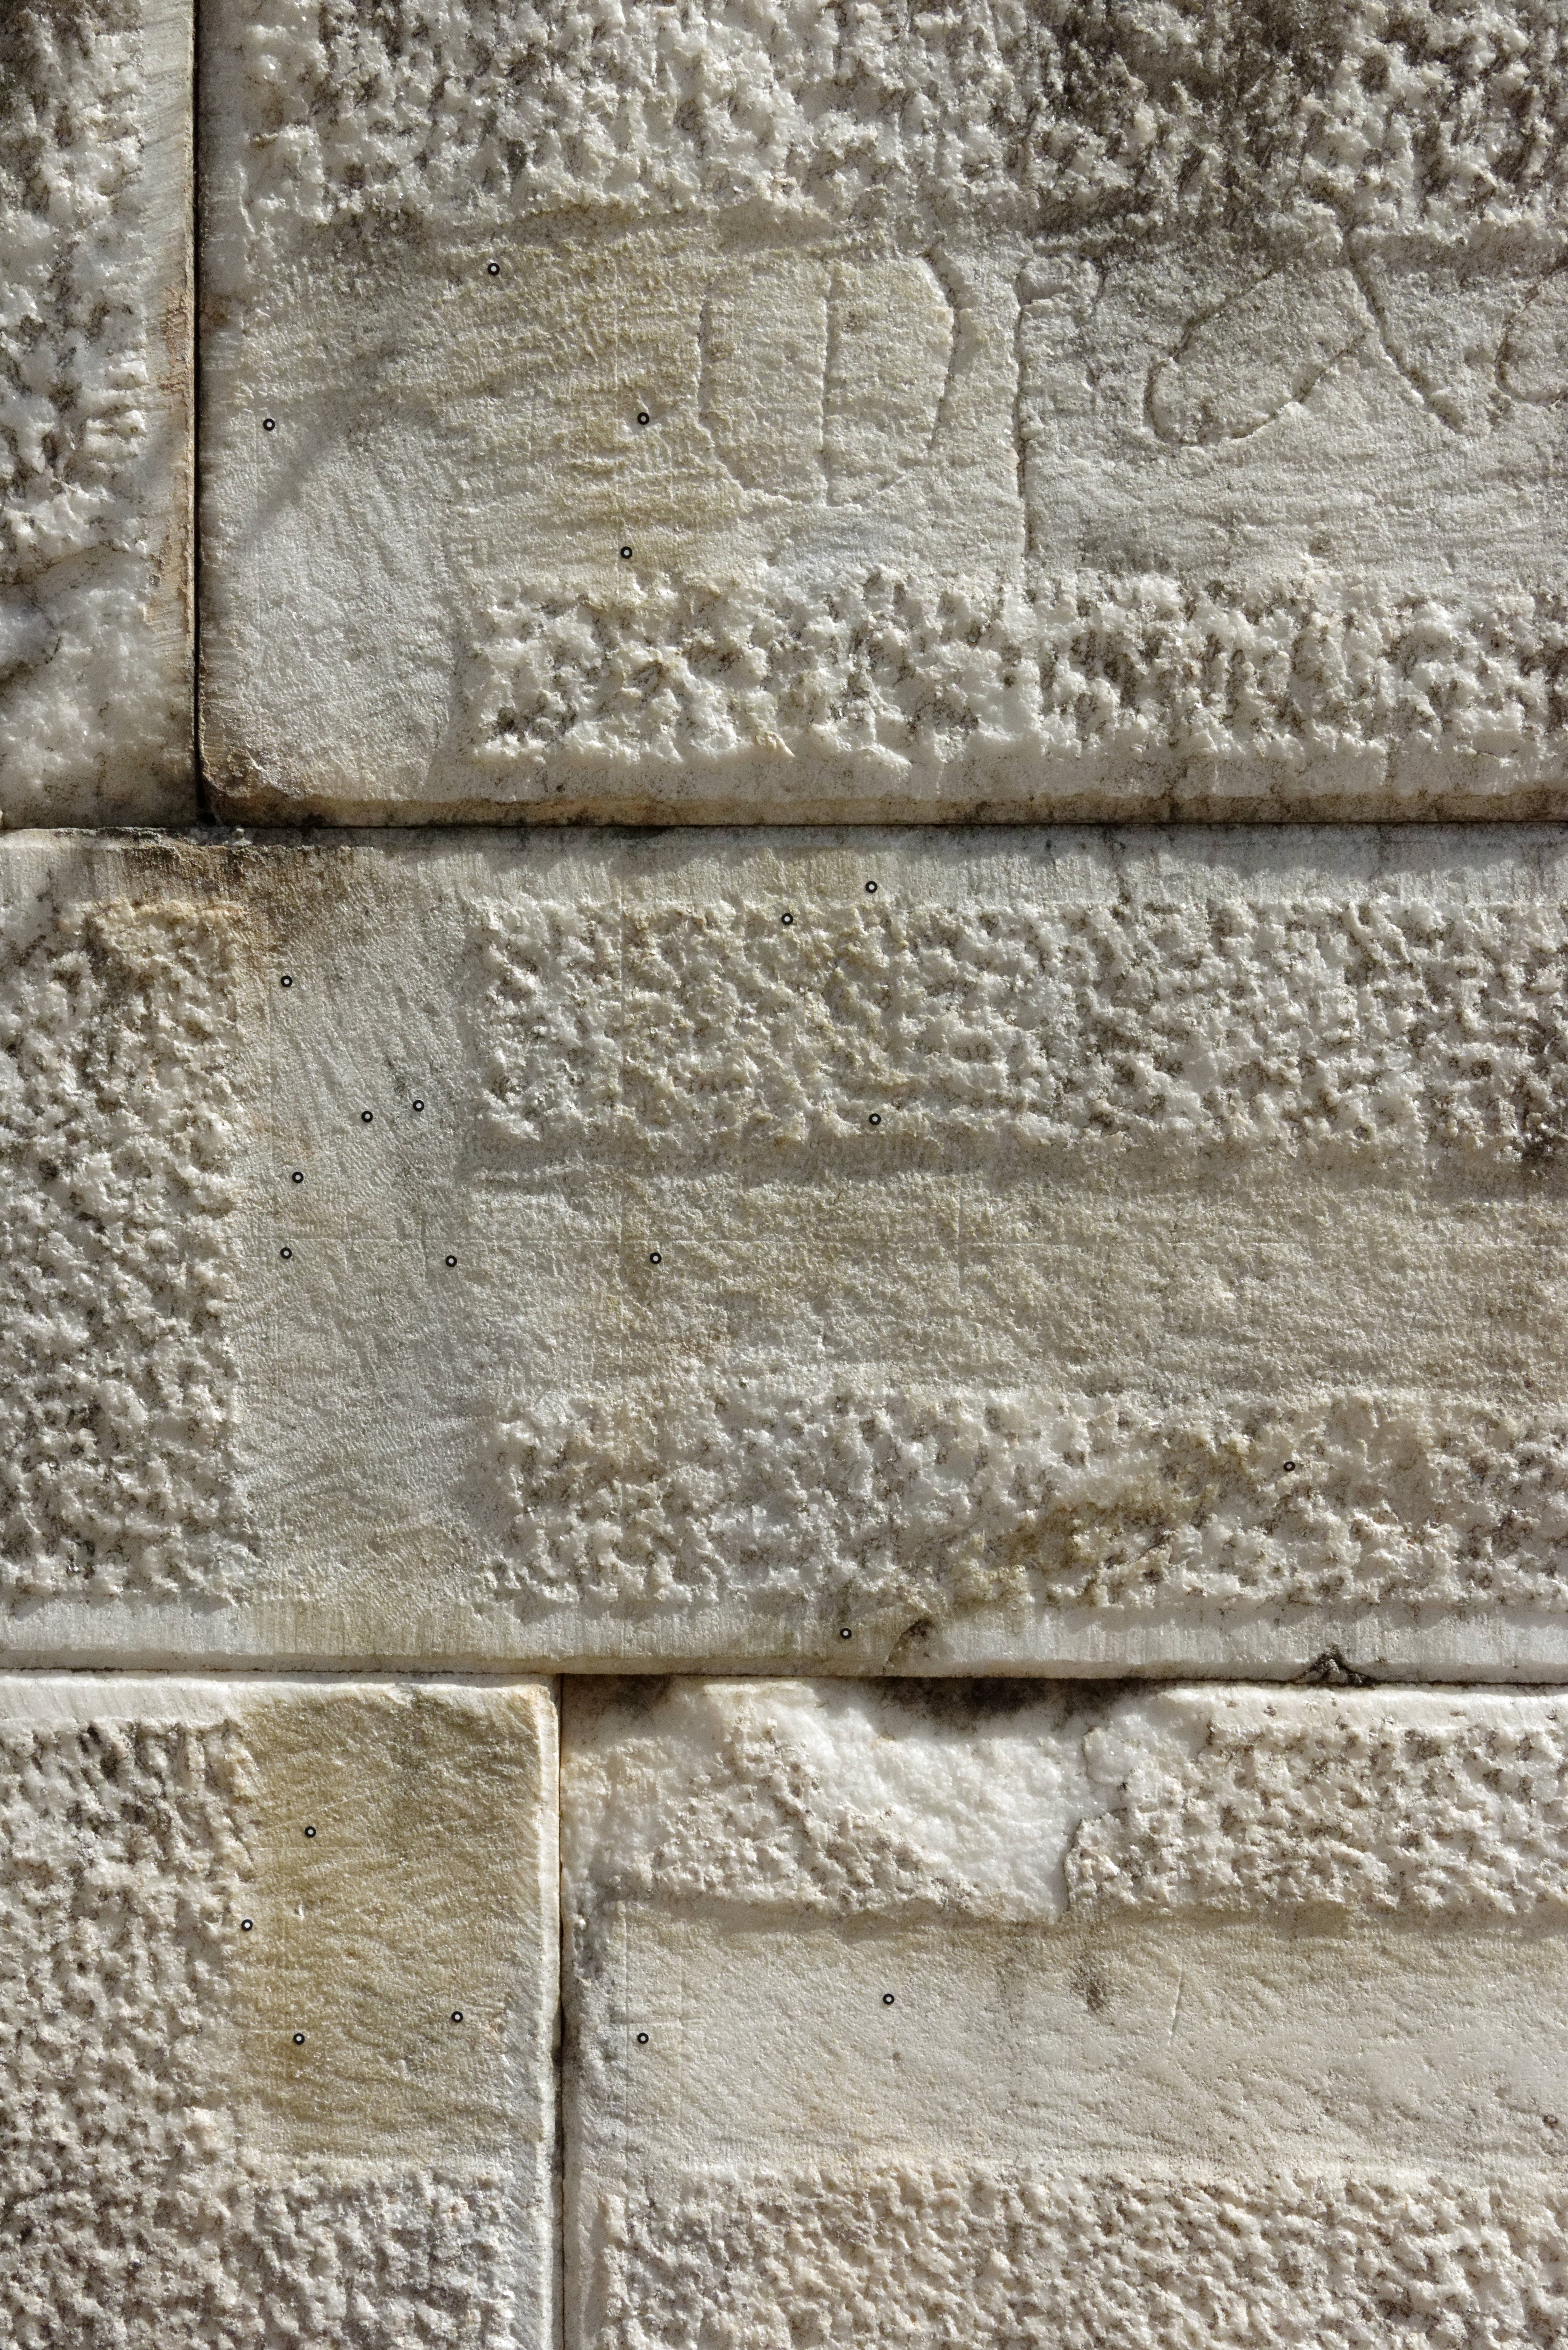
\includegraphics[width=0.9\linewidth]{figures/DSC_4221}
\caption{Linke Seite der Zeichnungsfläche}
\label{fig:DSC_4221}
\end{figure*}

\begin{figure*}[h]
\centering
\includegraphics[width=1.2\linewidth]{figures/ideal.png}
\caption{Aus Abb. \ref{fig:plot} rekonstruierte Säulenvorlage.}
\label{fig:plotideal}
\end{figure*}


Das Foto in Abb. \ref{fig:DSC_4221} zeigt die linke Seite der Zeichenfläche. Aus dem grob bearbeiteten Marmor sind die glatt geschliffenen Zonen für die Zeichnung eingelassen. Die Zonen erstrecken sich gerade über die Bereiche, die für die Zeichnung erforderlich sind. Kleine Markierungspunkte wurden vor Ort für die fotogrammetrischen Messungen aufgeklebt und hinterher rückstandsfrei entfernt. Wie in der Form eines großen Buchstabens E erstreckt sich die links begrenzende vertikale Zone über drei Marmorblöcke. Die horizontalen Zonen verlaufen über einige Blöcke hinweg nach rechts fast bis zum Eingangsbogen in den hinteren Theaterbereich. Der Handwerker muss vor der Herstellung der Zeichenzonen eine klare Vorstellung über die darin abzutragen Werkzeichnungen gehabt haben, da eine solche Bearbeitung des Marmors nicht rückgängig zu machen ist. An der langen Wandfläche findet sich auch keine vergleichbare bearbeitete Grundfläche. Die Markierungen selbst sind Einritzungen. Die vertikalen und insbesondere die horizontalen Linien müssen mit einem feinen Messer und Hilfsmitteln wie  Linealen sorgfältig in den Marmor eingeritzt worden sein. Die häufigen Markierungen wurden vermutlich mit einem gröberen Instrument eingeritzt und  haben eine unregelmäßige Linienführung, die auf eine Ausführung per Hand schließen lässt.

In einem ersten Schritt werden offensichtlich geometrisch zusammenhängende Zeichnungselemente als Konstruktionsgruppe zusammengeführt. Es sollen zunächst wenige, möglichst eindeutig zuzuordnende geometrische Objekte zu einer Konstruktionsgruppe zusammengestellt werden. Im weiteren Interpretationsverlauf kann sich ein solcher geometrischer Zusammenhang erweitern, aber auch revidiert werden. 

\subsection{Diagramm einer Säule}

In Abb. \ref{fig:plot} sind die Linien zuzüglich ihrer Länge zu sehen. 

\begin{description}
\item[1: Referenzlinie] Das erste offensichtliche Element ist die mittlere horizontale Strecke, die zwischen den ausgeprägten oberen und unteren horizontalen Strecke liegt und sorgsam gradlinig ausgeführt wird. Sie erstreckt sich zwischen der linken und rechten Vertikalen. Wobei die linke Vertikale scheinbar präzise rechtwinklig auf der mittleren horizontalen Strecke steht. Die rechte Vertikale steht gut sichtbar nicht rechtwinklig zur Referenzlinie.
\item[2: Obere horizontale Strecke]  Die obere horizontale Strecke beginnt nicht ganz im Anschluss an die vertikale Linie und verjüngt sich leicht nach rechts im ihrem Abstand zur horizontalen Referenzlinie. 
\item[3: Untere horizontale Strecke]  die untere horizontale Linie verläuft leicht verjüngend ebenso nach rechts bis zur rechten vertikalen Linie, jedoch nicht ganz symmetrisch zur oberen Linie.
\item[4: Rechte vertikale Linie] Die rechte vertikale Linie steht nicht senkrecht auf der Referenzlinie; sie schließt die Konstruktionsfläche nach rechts ab, liegt aber nicht parallel zur linken vertikalen Linie und hat eine unklare Funktion für die Konstruktion der Säule. Es entsteht der Eindruck, dass sie den Abschluss der zeichnerischen Konstruktion markiert, ohne dass sie für die Konstruktion wesentlich ist. Das erklärt auch, weshalb bei horizontalen Linien nicht bis zum Abschluss an der rechten vertikalen Strecke ausgeführt werden.
\end{description}

Auf den ersten Blick erscheint die Zusammenstellung der drei horizontalen Linien zusammen insbesondere mit der leicht schiefen rechten vertikalen Linie nicht sorgfältig ausgeführt. Die Asymmetrie der beiden leicht geneigten horizontalen Begrenzungslinien in Bezug auf die Referenzlinie lässt sich mit einfachsten Hilfsmitteln nachmessen.

In Abb. \ref{fig:screenshot010} sind die erfassten Linien in einem Vermessungstool abgetragen. Im unteren linken Bereich der Säulenkonstruktion sind intensive Markierungen vorgenommen worden. Die Bedeutung des Kreissektors wie auch die der vielen Markierungen ist noch nicht klar. Auch ist gut erkennbar eine weitere (kleinere) Säulenkonstruktion von rechts nach links abgetragen worden. Diese überlagert die Hauptzeichnung was möglicherweise auch die rechte vertikale Strecke als Sockelebene der zweiten Säule deuten lässt. Äußere horizontale Linien beginnen an der rechten vertikalen und neigen sich zur Referenzlinie bis zu der dritten vertikalen Strecke von links, die als Abschluss dieser zweiten Säulenkonstruktion zu verstehen ist. Wir konzentrieren uns im folgenden auf die Hauptlinien der von links nach rechts abgetragenen größeren Säule (siehe Abb. \ref{fig:plot}).  		
%\subsection{Modulare Einheit und Proportionen}
\section{Bauzeichnung und Säulenkonstruktion}

In Abb. \ref{fig:plotideal} ist die Säulenvorlage, die aus Abb. \ref{fig:plot} rekonstruiert wurde, zu sehen. 
Die Abstände zwischen den Eck- und Schnittpunkten A-F sowie die Winkel sind hier zusammengestellt:

\begin{itemize}
\item AB: 3.276 m
\item CD: 3.269 m
\item EF: 3.265 m
\item AC: 0.232 m
\item CE: 0.230 m
\item BD: 0.202 m
\item DF: 0.195 m
\item $\measuredangle{(AC u. AB)}$: $\mathrm{90.44}^\circ$
\item $\measuredangle{(AB u. CD)}$: $\mathrm{90.47}^\circ$
\item $\measuredangle{(DE u. EF)}$: $\mathrm{89.55}^\circ$
\end{itemize}

Folgende Proportionen sind auffällig:

\begin{itemize}
\item Verhältnis der Länge der Referenzlinie (CD) zur linken Vertikalen (AE): $\frac{3.269 \mathrm{m}}{0.462 \mathrm{m}}$ = 7.076
\item Verhältnis der linken Vertikalen (AE) zur rechten Vertikalen (BF) unter Berücksichtigung der \linebreak Schnittpunkte mit den Horizontalen: $\frac{0.462 \mathrm{m}}{0.397 \mathrm{m}}$  = 1.179 was mit einer Abweichung von ca. 3 $\%$ dem Verhältnis $\frac{8}{7}$ entspricht.
\end{itemize}

\section{3D Modell einer Säule}

\begin{figure*}[h]
\centering
\includegraphics[width=1\linewidth]{figures/FullMotion.png}
\caption{Verschiebung der y Komponente des Mittelpunktes aufgetragen auf die Referenzlinie.}
\label{fig:fullmotion}
\end{figure*}

\begin{figure*}[h]
\centering
\includegraphics[width=1\linewidth]{figures/CompareZR.png}
\caption{Verschiebung der Mittelachse der realen Säule (R) im Vergleich mit der Mittelpunktsverschiebung der aus der Zeichnung rekonstruierten Säule.}
\label{fig:compare}
\end{figure*}

\begin{figure*}[h]
\centering
\includegraphics[width=1\linewidth]{figures/Konstruktionsidee.png}
\caption{Mögliche Konstruktionsvorschrift.}
\label{fig:construction}
\end{figure*}



\subsection{Fundort}

\begin{figure*}[h]
	\centering
	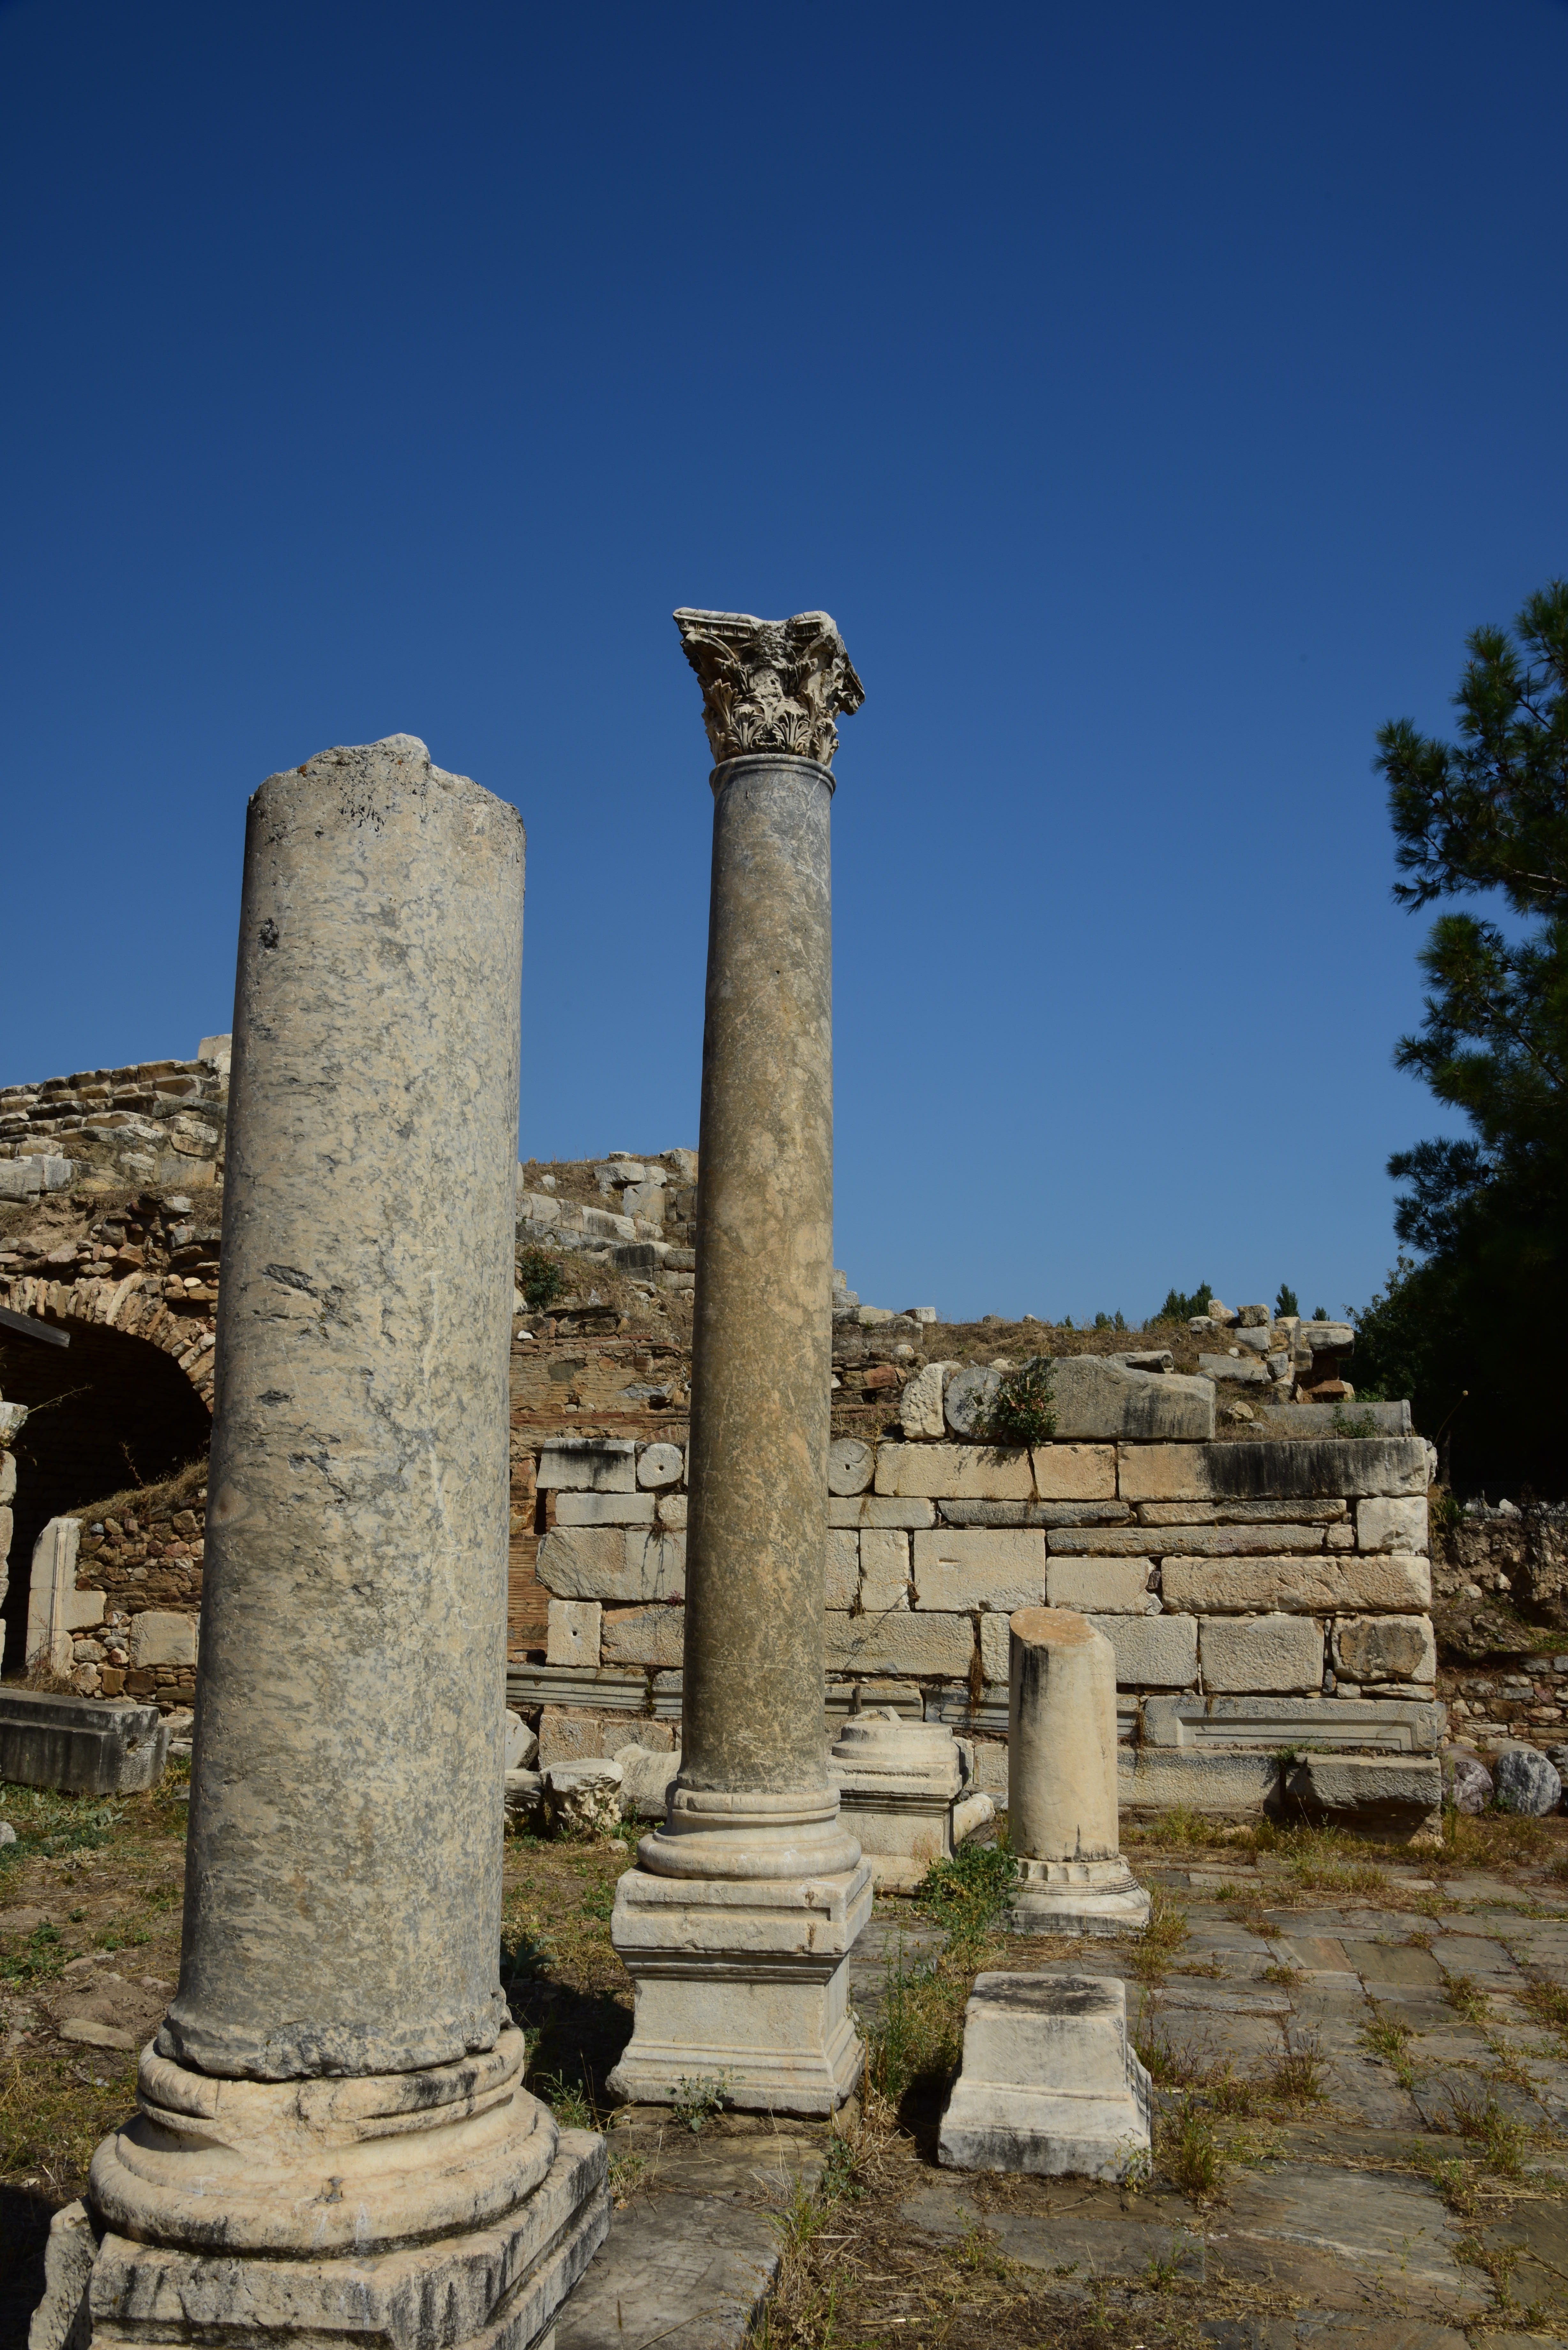
\includegraphics[width=1\linewidth]{figures/DSC3827.jpg}
	\includegraphics[width=0.7\linewidth]{figures/d1.JPG}
	\caption{Fotos der analysierten Säule an ihrem heutigen Aufstellungsort. Aus dem Betrachtungswinkel des linken Fotos erkennt man die schiefe linke Randlinie.}
	\label{dsc3827}
\end{figure*}

 Gleich ausserhalb des Theaters auf dem angrenzenden Gelände (in Abb. \ref{fig:screenshot002} bei Pos. 43) ist heute eine vollständig erhaltene Säule auf ihrem Sockel wieder aufgestellt. Der Standort scheint von den Archäologen plausibel gewählt, die Säule aber wurde neu aufgerichtet. Deshalb kann nicht davon ausgegangen werden, dass die Richtung der Asymmetrie der Säule der antiken Aufstellung entspricht. Die Säule besitzt ungefähr die Dimensionen der in der Bauzeichnung abgetragenen Hauptlinien, aber auch bei ihr ist eine Entasis zu erkennen, die es als Profilkurve in der Zeichnung nicht gibt. 


\begin{figure*}[h]
	\centering
	\includegraphics[width=1\linewidth]{figures/screenshot008}
	\caption{Positionen der Kameras um die rekonstrierten 3D Punktewolke}
	\label{fig:screenshot008}
\end{figure*}


\subsection{3D Rekonstruktion mit structure-from-motion}

Die Datengrundlage für die 3D Rekonstruktion der Säule \href{http://dx.doi.org/10.17171/2-2-36-1}{(\textit{doi:10.17171/2-2-36-1})} ist eine Serie von hochauflösenden Digitalfotos (Nikon D810) um beide Säulen herum (siehe \href{http://dx.doi.org/10.17171/2-2-10}{\textit{doi:10.17171/2-2-10}} und Abb. \ref{fig:screenshot008}). Die Geometrie der Säule wurde mit einem Laser Entfernungsmesser und einem Auflagemaßstab gemessen. Sie sind alternative Grundlagen für die Kalibrierung der 3D Modelle. 


\begin{figure*}[h]
\centering
\includegraphics[width=1\linewidth]{figures/screenshot007}
\caption{Rekonstruiertes 3D Modell der Säule in Meshlab}
\label{fig:screenshot007}
\end{figure*}


\begin{figure*}[h]
\centering
\includegraphics[width=0.7\linewidth]{figures/saeulenvergleich}
\caption{Vergleich der 3D Modelle, die mit unterschiedlichen Rekonstruktionsprogrammen nach der Structure-from-motion Methode errechnet wurden. Verglichen wurden die Modelle von Agisofts Photoscan mit denen von CaptureReality. Die Differenzen der Modelle wurden mit GOM verglichen. Auf der Farbscala sind verschiedene Abweichungen dargestellt. Die Differenzen liegen unterhalb einem Zehntel mm.}
\label{fig:saeulenvergleich}
\end{figure*}

%\subsection{Scalierung des Modells}

\subsection{Geometrie der Säule}

Auffällig ist die Geometrie der Säule, da diese nicht symmetrisch um ihre Mittelachse ist. Es ist ein Zylinder, mit einem leicht ellipsoiden Querschnitt. 
Weiterhin verschiebt sich (bei Annahme einer symmetrischen Entasis) der Mittelpunkt des Querschnittes vom Schaft zum Kapitell. Eine mögliche Erklärung wäre die im vorherigen Kapitel diskutierte Abweichung der Referenzlinie von der linken Vertikalen. Diskutiert werden soll, ob die leichte Neigung der Referenzlinie in der Bauzeichnung, genau die Verschiebung des Mittelpunktes erklären kann. Die 3D Modellierung mit  \texttt{Mathematica} zeigt die Verschiebung des Ellipsenschwerpunktes anhand von fünf ausgewählten Höhen der Säule, was in Abb. \ref{fig:figversch} illustriert ist. 


\begin{figure*}[h]
\begin{minipage}{.26\textwidth}
  \centering
  \includegraphics[width=1\linewidth]{figures/V3.png}
  %\caption{0.2 m}
  \label{fig:sfig1}
\end{minipage}%
\begin{minipage}{.26\textwidth}
  \centering
  \includegraphics[width=1\linewidth]{figures/V2.png}
  %\caption{0.6 m}
  \label{fig:sfig2}
\end{minipage}
\begin{minipage}{.26\textwidth}
  \centering
  \includegraphics[width=1\linewidth]{figures/V1.png}
  %\caption{1 m}
  \label{fig:sfig3}
\end{minipage}
\begin{minipage}{.26\textwidth}
  \centering
  \includegraphics[width=1\linewidth]{figures/V06.png}
  %\caption{2 m}
  \label{fig:sfig4}
\end{minipage}
\begin{minipage}{.26\textwidth}
  \centering
  \includegraphics[width=1\linewidth]{figures/V02.png}
  %\caption{3 m}
  \label{fig:sfig5}
\end{minipage}
\caption{Die Verschiebung des Ellipsenmittelpunktes als Funktion der Säulenhöhen 0.2 m, 0.6 m, 1 m, 2 m, 3m.}
\label{fig:figversch}
\end{figure*}

Die Verschiebung der y-Komponente stimmt genau mit der Abweichung der Referenzlinie überein (siehe Abb. \ref{fig:fullmotion}).

\subsection{Konstruktionsidee}

Wenn die Annahme stimmt, dass die Säule von Aphrodisias aus der Bauzeichnung konstruiert wurde, dann muss diskutiert werden, mit welchem Verfahren. 
Eine Idee wäre, dass die Konstruktionszeichnung auf jeder Seite des Quaders abgetragen wird, was in Abb. \ref{fig:construction} illustriert wird. Damit würden die obere und die untere Horizontale die Verjüngung der Säule vorgeben, während die Referenzlinie auf jeder Quaderseite einen Punkt des Ellipsenquerschnittes definiert. Insgesamt würden also vier Punkte für jeden Querschnitt der Höhe zur Verfügung stehen. Die Asymmetrie der oberen und unteren Horizontalen bezüglich einer "idealen" Referenzlinie würde dann die "Schiefe" der Säule definieren. 

Mit der Vorschrift aus jeweils vier Punkten einen Ellipsenquerschnitt zu erzeugen wurde aus der Zeichnung in  \texttt{Mathematica} ein 3D Modell erstellt.
Dieses 3D Modell wurde analog zum realen 3D Modell mit der selben Routine ausgewertet (siehe Abb. \ref{fig:figversch}). Das Ergebnis kann man in Abb. \ref{fig:compare} sehen. Die y-Komponenten der Mittelpunktsverschiebung für die reale und die Zeichungssäule stimmen sehr gut überein. 

\begin{figure*}
	\centering
	\includegraphics[width=1.6\linewidth]{figures/WandWeitereRelevanteLinien.pdf}
	\caption{Weitere relevante Linien. Die gestrichene Strecke beginnt links am unteren Punkt P1 und
		geht durch die auffällige mittlere Markierung "marker1". Bemerkenswert ist, dass diese Linie genau das Ende der oberen horizontalen Begrenzungslinie markiert.}
	\label{weitere}
\end{figure*}

\begin{figure*}[h]
\centering
\includegraphics[width=1.6\linewidth]{figures/screenshot010}
\caption{Alle aufgenommenen Markierungen in einem Vermessungstool. Im Bereich unterhalb der unteren Horizonalen sind die Vermessungsmarken des Tools zu sehen.}
\label{fig:screenshot010}
\end{figure*}

\begin{figure*}[h]
\centering
\includegraphics[width=1\linewidth]{figures/screenshot006}
\caption{Hauptlinien der Säulenzeichnung Aphrodisias in der Vermessung mit  \texttt{Mathematica}}
\label{fig:screenshot006}
\end{figure*}

%\bibliography{export}

\begin{backmatter}
	
	
	\section*{Author's contributions}
	 Gerd Graßhoff ist für die Gesamtkonzeption des Projekts und des Artikels verantwortlich. Gordon Fischer hat sich  mit der Datenauswertung und der Programmierung von  \texttt{Mathematica Notebooks} befasst.  Dem Exzellenzcluster Topoi EXC 264 danken wir für die Unterstützung im Rahmen der Forschergruppe D1 und D5.
	\section*{Acknowledgements}
	
	
	Bedanken insbesondere Bernhard Fritsch für die Unterstützung beim Aufbau des Repositorium der digitalen Quellen, die separat in der Edition Topoi publiziert werden.  Bei der fotografischen Bauaufnahme und der Vermessung der Referenzpunkte haben neben Gerd Graßhoff
	Joanna Pruszynska, Elisabeth Rinner und Anette Schomberg mitgewirkt.
	
	% if your bibliography is in bibtex format, use those commands:
	\bibliographystyle{vancouver} % Style BST file
	\bibliography{export}      % Bibliography file (usually '*.bib' )
	
	% or include bibliography directly:
	% \begin{thebibliography}
	% \bibitem{b1}
	% \end{thebibliography}
	
	%%%%%%%%%%%%%%%%%%%%%%%%%%%%%%%%%%%
	%%                               %%
	%% Figures                       %%
	%%                               %%
	%% NB: this is for captions and  %%
	%% Titles. All graphics must be  %%
	%% submitted separately and NOT  %%
	%% included in the Tex document  %%
	%%                               %%
	%%%%%%%%%%%%%%%%%%%%%%%%%%%%%%%%%%%
	
	%%
	%% Do not use \listoffigures as most will included as separate files
	
\end{backmatter}

\end{document}
